\chapter{Research objectives} \label{cha:Objectives}

\section{Research questions} \label{cha:Research-questions}
Published studies in the area of low-thrust trajectory optimisation, such as \textcite{Petropoulos2007}, frequently conclude that available optimisation techniques require further improvement. The most important question in this research project is how best to optimise a very-low-thrust trajectory. 

This project also provides a rare opportunity to actually test a low-thrust trajectory in orbit. Due to the prohibitive cost of space exploration, most studies of this nature are purely academic. Academic studies such as \textcite{Betts2000} often simplify or neglect the more awkward perturbing forces acting on the spacecraft such as solar wind and inhomogeneous gravity fields, for the sake of elegant mathematical solutions. The combination of very-low-thrust and the fact that the trajectory resulting from this study will actually be flown, requires that it take into account a much greater range of possible perturbations than most previous studies. The final launch will be greatly affected by the question of how significant these perturbations are, and particularly to what extent they may be exploited to reduce the effort needed to propel the spacecraft towards the Moon.

Furthermore, there are a number of very unique constraints on \BW. The thrusters produce substantially less thrust than modelled in most previous studies, resulting in a much tighter range of possible trajectories. The craft used in this program is also very limited by onboard power storage. This is yet another practical engineering issue barely considered in existing literature. Every few hours the craft must rotate to point its solar panels towards the Sun, and recharge its batteries. Once fully charged, it then rotates back to continue thrust vectoring for guidance control. Consequently the optimisation model must allow for variable thrust, including the ability to constrain thrust magnitude (to zero) at certain times. Developing a method to optimise intermittent thrust profiles like this will ensure the theoretical research of trajectory optimisation is applicable to real spacecraft.

\begin{figure}
\caption{A simplified trajectory for demonstration purposes early in the project.}
\label{fig:Early-trajectory}
\centering
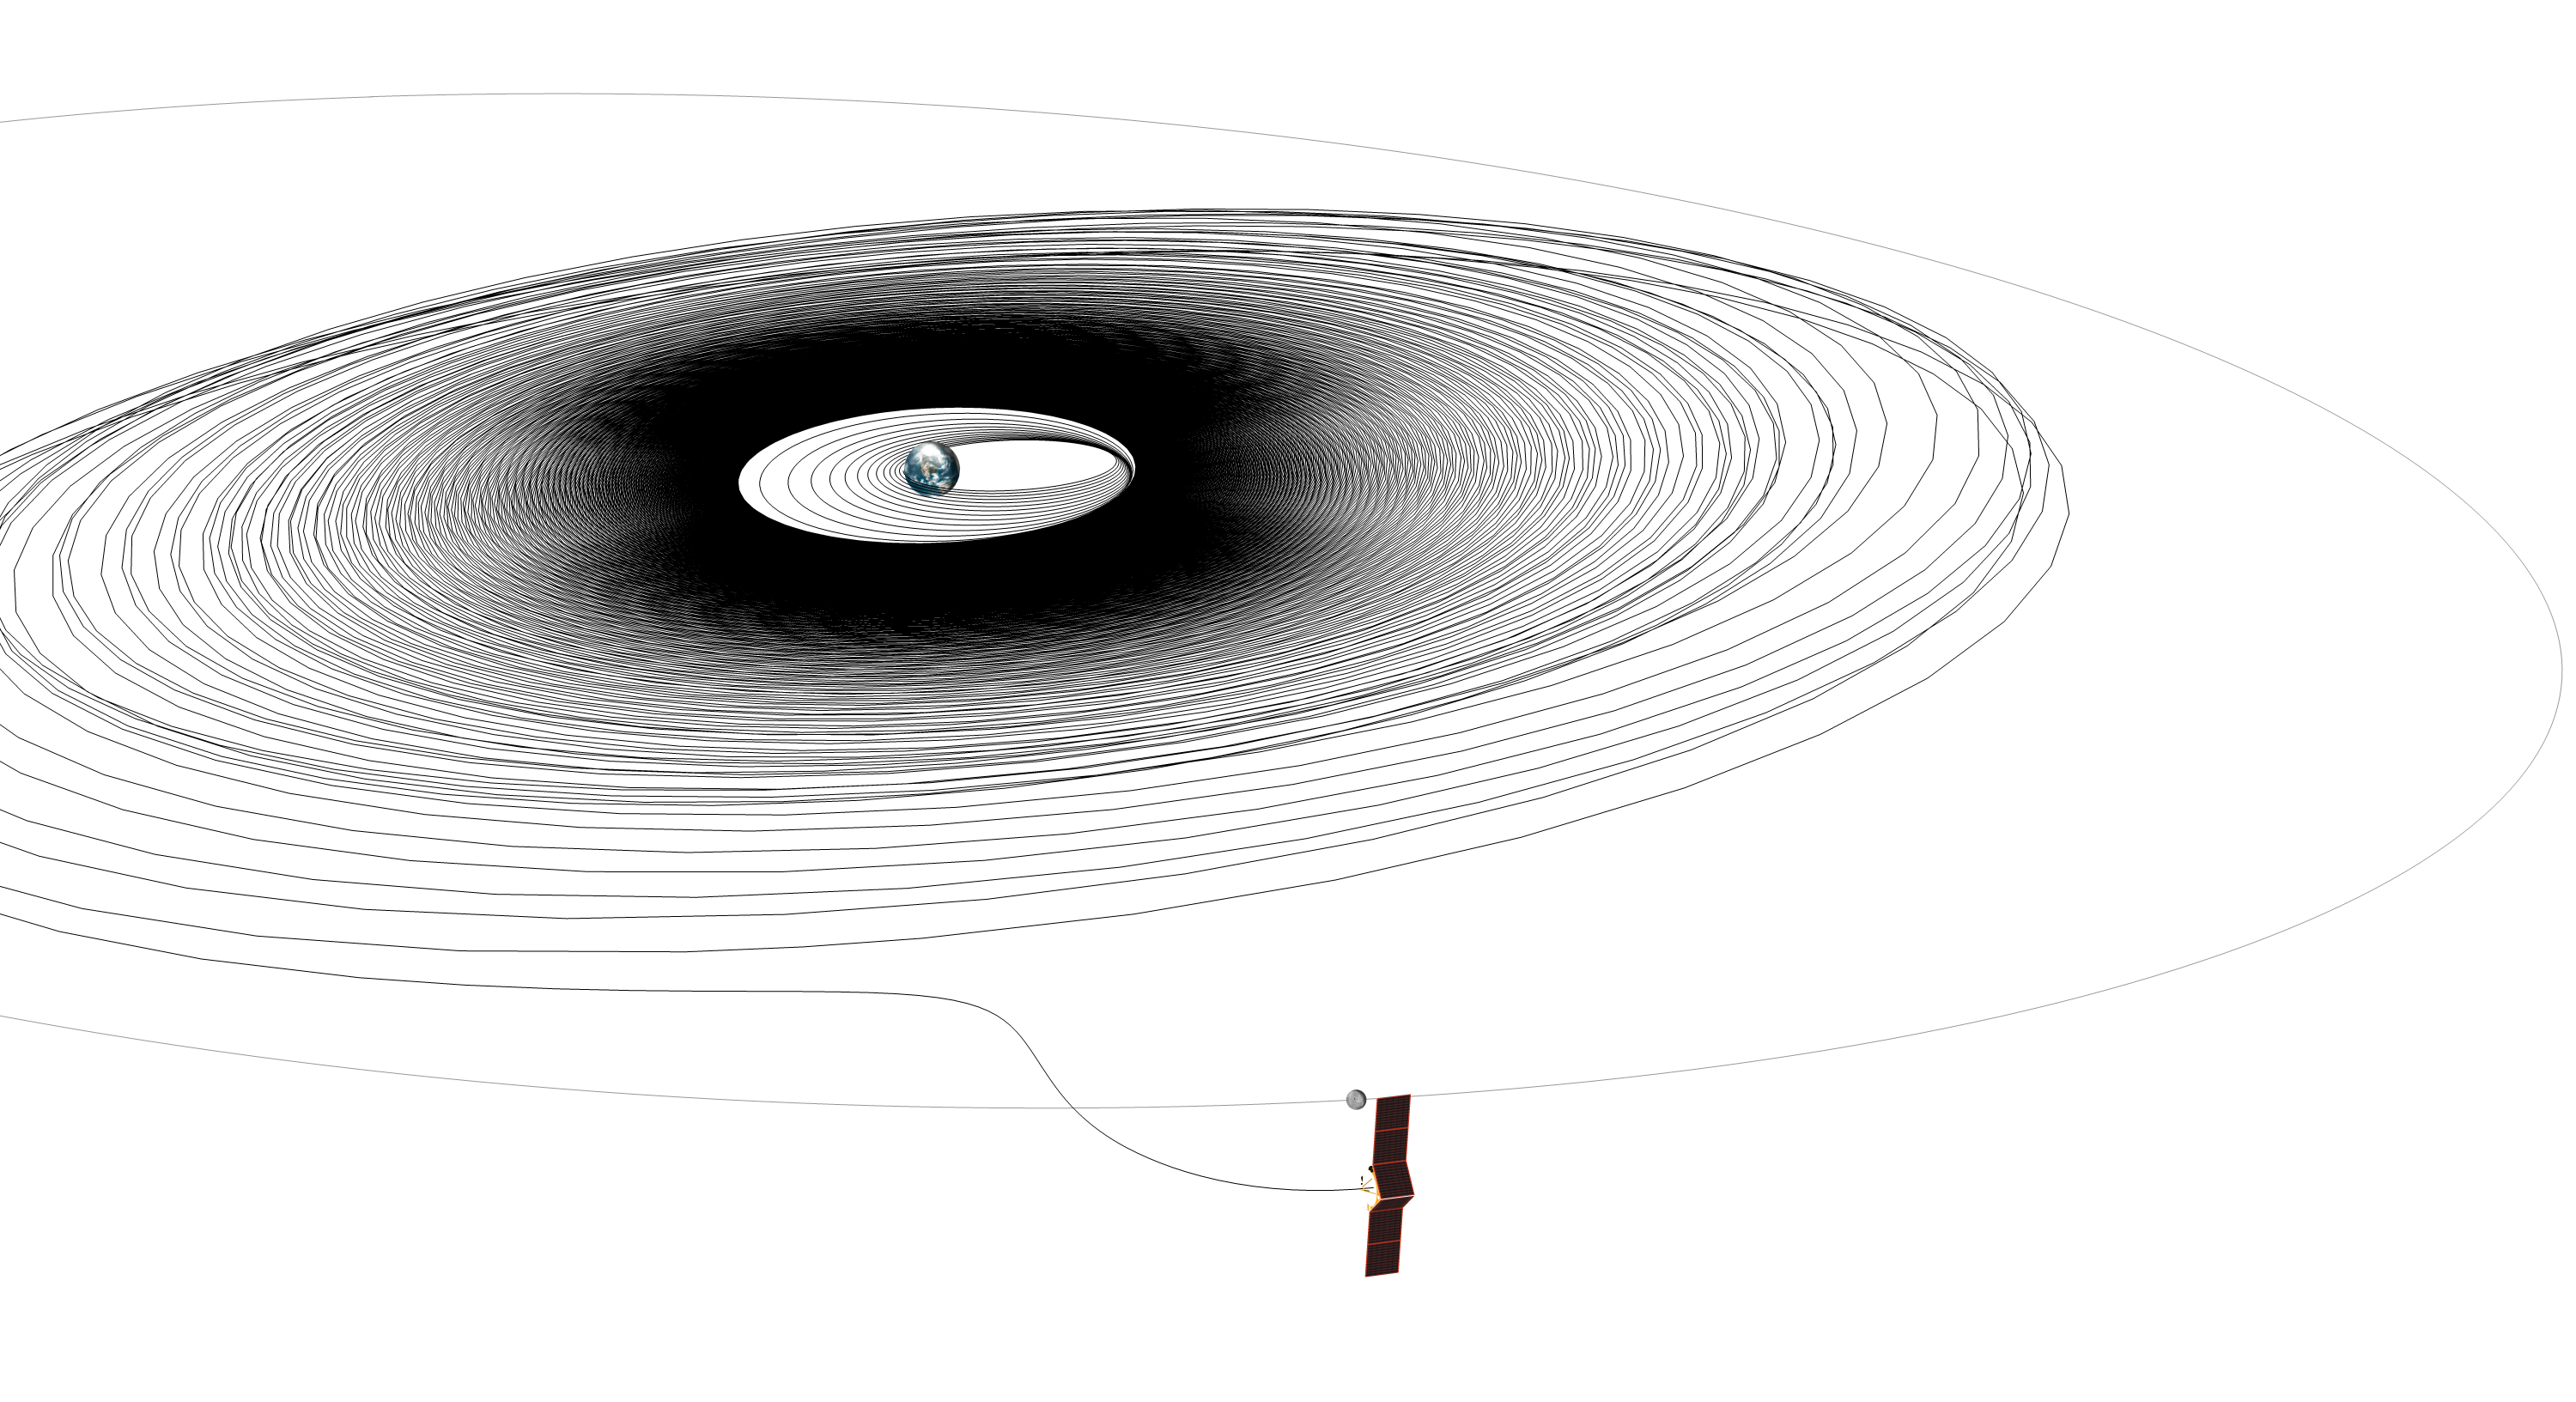
\includegraphics[width=\textwidth]{Images/BW1_Transfer.png}
\end{figure}

Other issues that were considered in this project, that have been neglected or ignored in most previous studies, include the spacecraft transiting through the Earth's shadow (eclipse), the possibility of varying the thrust level to conserve power, integrating the probable battery charge level throughout the transfer (based on sunlight received versus power used), intervals required for attitude control and reaction wheel desaturation and the amount of propellant required, and position monitoring and communication windows from the available groundstations. Many of these non-linear constraints have not been considered in previous studies, so the question of how to mathematically represent them such that they may be included in the optimisation is very important.

The primary objective of this project is to calculate a fuel-optimal trajectory for \BW. The research questions presented above may be summarised in two very interesting secondary outcomes of this project. Firstly, investigating the severity of perturbing forces on the spacecraft during transit, and to what extent they can be exploited. Secondly, developing a robust model to include a variety of non-linear trajectory constraints in the optimisation engine.

% Optimise trajectory
\section{Optimise very-low-thrust trajectory} \label{sec:Optimisation-objective}

This broad objective was broken down into the following tasks.

\begin{enumerate}
  \item Derive an appropriate model for the spacecraft, moving within a realistic space environment.
  \item Examine optimisation techniques and select one appropriate to this scenario.
  \item Explore different initial guesses for the optimisation, based on knowledge of orbital mechanics and exploitation of perturbing forces.
  \item Apply non-linear constraints to the optimisation.
\end{enumerate}

% Orbital mechanics
\subsection{Modelling} \label{sub:Modelling-task}

A complete description of the spacecraft and space environment model is presented in \autoref{cha:Orbital-dynamics-and-modelling}. Although there are multiple solutions available for each modelling hurdle, there are fairly well established best-practice solutions for the high fidelity modelling required over the long durations associated with low-thrust missions.

% Optimisation techniques
\subsection{Optimisation techniques} \label{sub:Optimisation-techniques}

Optimisation techniques suitable for trajectory optimisation were examined. Reviewed literature repeatedly cited the inadequacies of existing search methods as a major problem with existing optimisation methods (one such example is presented by \textcite{Petropoulos2007}, whom acknowledged a deficiency in the global search component of their optimisation routine). In particular, it was noticed that previous optimisations generally ignore non-linear thruster constraints, due to the additional complexity and stiffness they add to the optimisation problem. Therefore it was necessary to find a technique to model these constraints linearly. \textcite{Gao2008} presented a very promising variable thrust profile model that formed the basis of this technique. Other non-linear constraints listed in Section \ref{cha:Research-questions} were rarely if ever modelled in the existing literature, so finding a computationally efficient way to include them was essential to the suitability of the optimisation techniques used for this mission.
 
A thorough review of optimisation techniques is presented in Section \ref{cha:Optimisation}.

% Initial guesses
\subsection{Initial guesses} \label{sub:Initial-guesses}

Most optimisation techniques require an initial guess of the solution to be input into the algorithm, from whence it can improve some objective function. Existing search methods often have strong dependencies on the initial guess, as outlined frequently in literature such as \textcite{Dachwald2005}. Consequently it was important to investigate the performance of the optimisation under a variety of initial guesses. Based on orbital mechanics theory, a number of potentially optimal scenarios were investigated, as addressed in \autoref{cha:Discussion-of-results}. These were then compared to a number of randomly chosen initial guesses, to determine the breadth of the basin of convergence and the ability of the optimiser to handle multiple basins. Additionally a number of severely sub-optimal initial guesses were examined.

% Model nonlinear constraints
\subsection{Model non-linear constraints} \label{sub:Model-non-linear-constraints}

A highly simplified low-thrust lunar trajectory was developed. This assisted in developing an initial guess for the final optimisation. From this state, the optimiser was developed to include more complex constraints. Firstly coast phases were introduced to the existing constant-thrust profile, producing a bang-bang control scenario. Then the length of these coasting and thrusting phases was released, followed by the magnitude of the thrust. The electric charge consumed during a thrust phase was modelled, with the constraint that it cannot drop below zero. An approximation of charge gained by the solar panels was implemented, and then improved based on sunlight angle of incidence, Earth shadow and solar panel decay. This technique identified coasting phases required for recharging the spacecraft, providing constraints on the Attitude and Orbital Control System (AOCS). Based on the electric charge model, propellant use was modelled. Reaction wheel desaturation will be required to improve the fuel usage model, although this improvement is dependent on other project members working on the AOCS.

% Investigate perturbations
\section{Investigate perturbations} \label{sec:Perturbation-objective}

Once a robust model was developed for the trajectory optimisation, the impact of perturbations to the trajectory was investigated. This objective was required to highlight two major characteristics of the trajectory: firstly, the robustness of the trajectory in the event of unanticipated perturbations, and secondly whether anticipated perturbing forces may be exploited to propel the spacecraft.

The sensitivity of the trajectory was examined by introducing deterministic and stochastic inputs into variables such as the thrust angles, magnitudes, and gravitational perturbations, to simulate errors in the spacecraft control system, non-linearities in the thruster output, or unknown gravitational influences, to ensure that the proposed theoretical thrust regimes are applicable to real-world spacecraft. The magnitude of these error inputs was determined through consultation with experts on each of the sub-systems, as a percentage of the intended input. Additionally, the trajectory was simulated with errors of increasing magnitude to determine mission failure scenarios. Contingency trajectories will have to be determined for these cases, such as a single engine failure.

Anticipated, predictable perturbing forces may be used to help propel the spacecraft towards the Moon. It is well known from interplanetary trajectories such as those presented by \textcite{Petukhov2007} that a large amount of propulsive effort can be saved by exploiting gravitational assists. Some textbooks, such as \textcite{Kemble2006}, and other publications such as \textcite{Letterio_thesis} discuss the possibility of exploiting the Moon's gravity in a series of lunar \enquote{resonances} to assist a low thrust lunar transfer. Anticipated perturbations such as this are implicitly exploited by the optimiser since they do represent optimal scenarios, however due to imperfections in optimisation algorithms the initial guess strongly affects whether the gravitational assist is found.

% Investigate nonlinear constraints
\section{Investigate non-linear constraints} \label{sec:Constraint-objective}

As additional constraints and non-linearities were progressively added to the model, the impact of each constraint on the behaviour of the optimisation process was investigated to determine its effect on both the optimisation process and the resultant optimal trajectory. Optimal intermittent thrust profiles were compared with results for a comparable continual thrust profile to demonstrate the improvement (for example, thrusting twice as much at periapsis and then coasting compared to thrusting continuously throughout the orbit). 

\section{Scope}

It was anticipated that by judiciously choosing the thrust phases, the fuel efficiency could be improved. However, there are always limitations to such a project. The optimal thrust profile for this mission is very closely tied with the Attitude and Orbital Control System (AOCS). This provides further constraints on the project, and adds another whole level of modelling complexity. 

However, the AOCS for \BW\ is still being finalised and will be tested on the forthcoming test satellites \emph{Flying Laptop} and \emph{Perseus}. Consequently modelling and optimising the AOCS is beyond the scope of the project. Throughout this thesis it is assumed that the AOCS can provide the attitude required, when required, for as long as required. A corrollary of this assumption is that the spacecraft may be modelled as a point mass. Another consequence is that reaction wheel saturation cannot yet be predicted. Thus reaction wheel desaturation could not be included in this project, although given the rotation rate of 1\degrees\ per second specified in the design it is anticipated that the time required to reorient the spacecraft will have minimal effect on the thrust profile, and that reaction wheel desaturation can  easily be scheduled into the trajectory at a later date.

% Summary
\section{Summary of research objectives} \label{sec:Objective-summary}

Several fundamental objectives have been outlined for optimising the trajectory of \BW. These objectives include establishing reliable modelling and optimisation techniques within the Institute for Space Systems, determining efficient ways to model the non-linear forces present on an exo-atmospheric trajectory, and investigating how significant those forces are over the course of the the trajectory. Establishing some ground rules for practically optimising the trajectory of a spacecraft in this manner will improve the existing knowledge of low-thrust spacecraft trajectories.